\subsubsection{\theoryC{Dissecting heavy diphoton resonances}}
\contributors{B. Allanach, D. Bhatia, A. Iyer}
%{\bf Author(s): B. Allanach$^1$, D. Bhatia$^2$ and A. Iyer$^3$}\\
%$^1$ DAMTP, University of Cambridge, CMS, Wilberforce Road, Cambridge, CB3 0WA, United Kingdom email: {\tt B.C.Allanach@damtp.cam.ac.uk}\\
%$^2$ Department of Theoretical Physics, Tata Institute of Fundamental Research,
%Homi Bhabha Road, Colaba, Mumbai 400 005, India, email: {\tt disha@theory.tifr.res.in}\\
%$^3$ INFN-Sezione di Napoli, Via Cintia, 80126 Napoli, Italia, email: {\tt iyera@na.infn.it} 

We examine the phenomenology of the production of a heavy resonance $X$, 
which decays via other new on-shell particles $n$ into multi- (i.e.\ three
or more) photon final states.  In the limit that $n$ has a much smaller mass than $X$, 
the multi-photon final state may dominantly appear as a two photon
final state because the $\gamma$s from the $n$ decay are highly
collinear and remain unresolved.
We discuss how to discriminate this scenario
from $X \rightarrow \gamma \gamma$: rather than discarding non-isolated
photons, it is better instead to relax the isolation criterion and instead
form photon 
jet substructure variables. 
The spins of $X$ and $n$ leave their imprint upon
the distribution of pseudorapidity gap $\Delta \eta$ between the apparent two
photon 
states. In some models, the heavy resonance $X$ may decay into $nn$ or $n \gamma$, where
$n$ is an additional light
particle,
may further decay into photons leading to a multi-photon\footnote{In the
  present paper, whenever we refer to multi-photon final states, we refer to
  three or more photons.} final state. 
Examples of such models include hidden
valley models~\cite{Strassler:2006im,Strassler:2006ri}, the
NMSSM~\cite{Ellwanger:2009dp} or Higgs portal
scenarios~\cite{Schabinger:2005ei}. 
Describing angles in terms of the pseudorapidity $\eta$ and the azimuthal
angle around the beam $\phi$, the angular separation between two photons may be 
quantified by $\Delta R=\sqrt{(\Delta \eta)^2+(\Delta \phi)^2}$. 
Neglecting its mass, 
the opening angle between the two photons coming from a highly boosted
on-shell $n$ is 
\begin{equation}\Delta  R=\frac{m_n}{\sqrt{z(1-z)}p_T(n)},
\end{equation} purely from kinematics (this was
  calculated already in the context of boosted Higgs to $b \bar b$
  decays~\cite{Butterworth:2008iy}),
  where $z$ and 
 $(1-z)$ are  the momentum fractions of the photons\footnote{The decay is
   strongly peaked towards the minimum opening angle $\Delta R=2
   m_n/p_T$~\protect\cite{Chala:2015cev}.}. 
 Thus,
\begin{equation}
\Delta R = \frac{m_n}{M_X}\frac{2 \cosh \eta(n)}{\sqrt{z(1-z)}}. \label{eq:dRest}
\end{equation}
In the limit $m_n/M_X\rightarrow 0$, $\Delta
R\rightarrow 0$ and the two photons from $n$ are 
collinear, appearing as one photon; thus several possible interpretations
can be ascribed to an apparent diphoton signal.

We assume that any couplings of new particles such as the $X$ (and the $n$, to
be introduced later) to Higgs
fields or $W^\pm, Z^0$ bosons are negligible. 
\eq{eq:Lagrangian1} gives an effective field theoretic interaction
Lagrangian for the 
coupling of $X$ to a pair of photons, when $X$ is a scalar (first line) or  a
graviton (second line). 
 \begin{eqnarray}
	\mathcal{L}_{X={\rm spin~0}}^{int} &=&    - \eta_{GX}\frac{1}{4} G_{\mu \nu}^a
                                   G^{\mu \nu a} X  - \eta_{\gamma X} \frac{1}{4}
                                   F_{\mu \nu} F^{\mu \nu} X, \nonumber\\
	\mathcal{L}_{X={\rm spin~2}}^{int} &=&    -\eta_{T\psi X}T_{fermion}^{\alpha\beta}
                                   X_{\alpha\beta}-\eta_{TGX} T_{gluon}^{\alpha\beta}
                                   X_{\alpha\beta}  - \eta_{T\gamma X} 
T_{photon}^{\alpha\beta} X_{\alpha\beta}.
	\label{eq:Lagrangian1}
\end{eqnarray}
where  $T^{\alpha\beta}_i$ is the stress-energy tensor for the  field $i$
and the $\eta_j$ are effective couplings of mass dimension -1.
$F_{\mu \nu}$ is the field strength tensor of the photon (this may be obtained
in a SM invariant way from a coupling involving the field strength tensor of
the hypercharge gauge boson),
whereas $G_{\mu 
  \nu}^a$ is the field strength tensor of a gluon of adjoint colour index $a
\in \{ 1,\ \ldots , 8 \}$.
As noted earlier, the direct decay of a vector boson into two photons is
forbidden by the 
Landau-Yang theorem~\cite{Landau:1948kw,Yang:1950rg}. 

Although we assume that $n$ is electrically neutral, it may decay to two
photons through a loop-level process (as is the case for the Standard Model
Higgs boson, for instance). 
Alternatively, if $X$ is a spin 1 particle, it could be produced by
quarks in the proton and then decay into $n \gamma$. 
The Lagrangian terms would be
\begin{equation}
\mathcal{L}^{int}_{X\,={\rm spin~1},n}= -
                                     (\lambda_{\bar q X q} \bar q_R \gamma_\mu
                                     X^\mu q_R
 + \lambda_{\bar Q X Q} \bar Q_L \gamma_\mu X^\mu Q_L + H.c.)
-\frac{1}{4}\eta_{nX\gamma}
                                     n{\tilde X}_{\mu\nu}F^{\mu\nu},
                                     \label{eq:wouldbe}
\end{equation}
where  $\lambda_i$ are  dimensionless
couplings, $q_R$ is a right-handed quark, $Q_L$ is a left-handed quark doublet
and ${\tilde X}_{\mu \nu}=\partial _\mu
X_\nu - \partial_\mu X_\nu$. 
The decay $X_{spin=1}\rightarrow n \gamma$ would
have to be a loop-level process, as explicitly exemplified in
\citeref{Chala:2015cev}, since electromagnetic gauge invariance 
forbids it at tree level. 
The possible different spins involved in multi-photon production processes, along with our nomenclature for them, are listed in \tabb{tab:cases}. 
\begin{table}\begin{center}
\begin{tabular}{|c|c|}\hline
Model & Process \\ \hline
$S2$ & $pp \rightarrow S \rightarrow \gamma \gamma$ \\
$S4$ & $pp \rightarrow S \rightarrow nn \rightarrow \gamma
       \gamma+\gamma\gamma$ \\ 
$V3$ & $pp \rightarrow Z' \rightarrow n \gamma \rightarrow \gamma + \gamma
       \gamma$ \\
$G2_{ff}$ & $q \bar q \rightarrow G \rightarrow \gamma \gamma$ \\ 
$G4_{gg}$ & $gg \rightarrow G \rightarrow nn \rightarrow \gamma \gamma+\gamma
            \gamma$ \\
$G4_{ff}$ & $\bar q q \rightarrow G \rightarrow nn \rightarrow \gamma \gamma+\gamma
            \gamma$ \\
\hline
%          \includegraphics[width=8cm]{cases.pdf}
\end{tabular}
\end{center}
\caption{\label{tab:cases} Cases to discriminate with a scalar $n$ and a heavy
resonance which is: scalar ($S$), spin 1 ($Z'$) or spin 2 ($G$). We have
listed the main signal processes to discriminate between in the second column,
ignoring any proton remnants. The notation used for a given model is $Xk$:
$X=S,V,G$ labels the spin of the resonance and $k$ denotes the number of
signal photons at the parton level in the final state.} 
\end{table}
The first tool for model discrimination is the photon sub-jet variable $\lambda_J=\log(1-p_{T_L}/p_{T_J})$, where $P_{T_L}$ denotes the transverse momentum of the leading photon sub-jet whilst $p_{T_J}$ is the transverse momentum of the whole photon jet. Double pronged photon jets have a peak at $\lambda_J=-0.3$. This may be observed when the signal is multi-photon and $m_n$ is not too small, as \fig{fig:lambdaj} shows.
\begin{figure}
\begin{center}
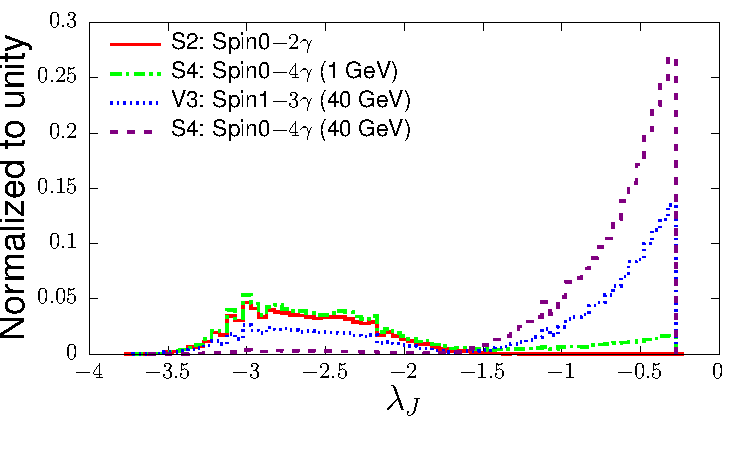
\includegraphics[width=0.45 \textwidth]{\main/section7OtherSignatures/img/plot-lambda.pdf}
\caption{Distribution of $\lambda_J$ variable for various signal hypotheses. $m_n$ is noted in parentheses in the legend for the relevant cases.\label{fig:lambdaj}}
\end{center}
\end{figure}

Here, we neglect backgrounds and only focus on the signal. This is a good approximation for heavy resonances where backgrounds die off exponentially with invariant mass of the apparent diphoton pair, provided that the signal cross-section is large enough. The signal cross-section is of course set by the size of the couplings in \eqs{eq:Lagrangian1} and \eqref{eq:wouldbe}, which may be adjusted as required. Here, we consider one of the cases in \tabb{tab:cases} at a time, with cross-sections of all other cases set to zero. 

If there is a sizable peak at $\lambda_J=-0.3$, the model possibilities are $S4,V3,G4_{gg}$ and $G4_{ff}$. Further to this, $V3$ may be further discriminated owing to its double peak structure: at $\sim$-3 and at -0.3. We call this case A.
If there is no sizable peak, we can either have $S2$ or $m_n$ very small. This latter case we call case B.

After categorization into case A or B, we can use the fact that
each case in Ref.~\ref{tab:cases} corresponds to a different distribution in $\Delta \eta$, the difference in pseudo-rapidity between the two initially identified photons.
We plot the $\Delta \eta$ distributions for the different spin cases in \fig{fig:deta}. 
\begin{figure}
\begin{center}
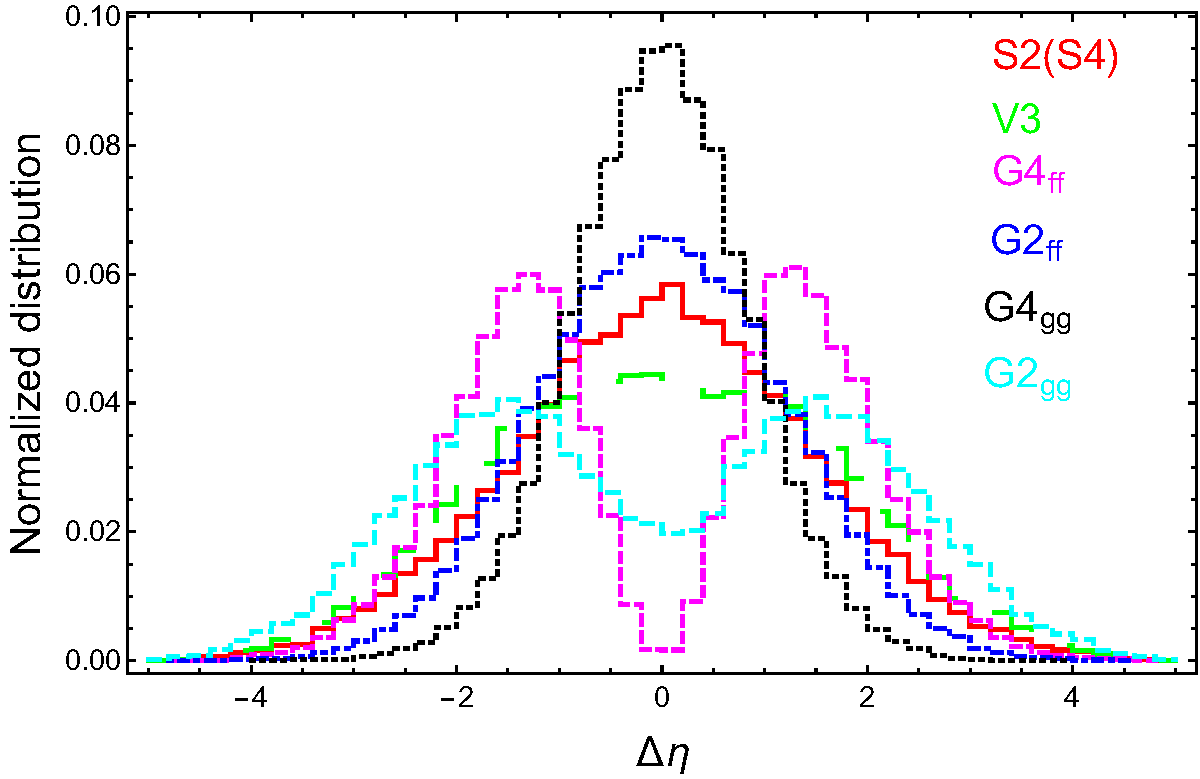
\includegraphics[width=0.45 \textwidth]{\main/section7OtherSignatures/img/del-eta-27TeV.pdf}
\caption{Signal $\Delta \eta$ distribution for various different spin combinations at $\sqrt{s}=27$ TeV, $m_X=2.5$ TeV. The cases S2 and S4 are practically indistinguishable by eye and so we only plot one histogram for them. \label{fig:deta}}
\end{center}
\end{figure}
We calculate $N_R$, the expected number of signal events required to disfavor a hypothesis $H_S$ over another hypothesis $H_T$ to an odds factor of $R=20$ from the $\Delta \eta$ distributions in the 
discretized Kullback-Leibler 
method proposed in \citeref{Allanach:2017qbs}.
\begin{table}[h!]
	\begin{center}
		\begin{tabular}{|c|c|c|c|c|} 
			\hline
			
			$N_R$  & Ecm         & $S4$   & $G4_{gg}$ &  $G4_{ff}$ \\ \hline
			\hline
			
			$S4$   & 14 TeV       &$\infty$&23&12\\    
			& {27 TeV} &$\infty$&17&8 \\ \hline \hline
			
			$G4_{gg}$  & 14 TeV   &34&$\infty$&5\\  
	&{27 TeV}			 &24&$\infty$&3\\ \hline \hline 
			$G4_{ff}$ & 14 TeV    &18&5&$\infty$ \\  
			& {27 TeV} &11&4&$\infty$ \\ \hline  \hline    
		\end{tabular}
		\caption{\label{tab:tab:spindiscrimination1lambda} Spin discrimination in case A: $N_R = {\mathcal L}
			\sigma_{tot}^{(X)}$, the expected
			number of total signal events required to be produced 
			to discriminate against the `true' row
			model versus a column model by a factor of 20
			for $m_n=100$ GeV.} 
	\end{center}
\end{table}
\begin{table}[h!]
	\begin{center}
		\begin{tabular}{|c||c|c|c|c|c|c|c|c|} 
			\hline
			$N_R$  & Ecm     & $S2$    & $S4$ & $V3$ & $G2_{gg}$ & $G4_{gg}$ & $G2_{ff}$ & $G4_{ff}$ \\ \hline
			\hline
			$S2$  & 14 TeV     & $\infty$&$19270$     &198&25&13&85&12  \\  
			      & {27 TeV}     & $\infty$ & 8676 & 269 & 26 & 16 & 92 & 14  \\ \hline \hline  
			$S4$  & 14 TeV     &  $19256$   &$\infty$ &202&25&13&81&13\\   
		& { 27 TeV}	&  8713   & $\infty$  & 311 & 28 & 15 & 83 & 14\\ \hline  \hline  
			$V3$  & 14 TeV     & 186  & 190  & $\infty$  & 55 & 7 & 30 & 19 \\  
& { 27 TeV}			& 261   & 299 & $\infty$ & 51 & 10 & 40 & 20 \\ \hline \hline  
			$G2_{gg}$& 14 TeV  &  28    &28&66&$\infty$ &4&11&35      \\  
		& { 27 TeV}	& 31  & 33 & 63 & $\infty$ & 5 & 13 & 41      \\ \hline \hline  
			$G4_{gg}$& 14 TeV  &   21   &21&12&6&$\infty$ &47&4\\  
		&{ 27 TeV} &  26   & 25 & 16 & 7  & $\infty$ & 55 & 5\\ \hline  	\hline  
			$G2_{ff}$& 14 TeV  &   101   &97&37&11&33&$\infty$ & 8   \\  
		& { 27 TeV} &  103  & 93 & 46 & 12 & 39 &$\infty$ & 9   \\ \hline 	\hline  
			$G4_{ff}$& 14 TeV  &   18   &18&26&36&4&12&$\infty$ \\     
		& { 27 TeV} &  19   & 20 & 29 & 41 & 5 & 13 &$\infty$ \\ \hline\hline  
		\end{tabular}
		\label{tab:spindiscrimination}
	\end{center}
	\caption{Spin discrimination for case B: $N_R = {\mathcal L}
		\sigma_{tot}^{(X)}$, the expected
		number of total signal events required to be produced 
		to discriminate against the `true' row
		model versus a column model by a factor of 20 at the 14 TeV
		LHC for $m_n=10$ GeV. \label{tab:two}} 
\end{table}
From Tables~\ref{tab:tab:spindiscrimination1lambda},\ref{tab:two}, we see that our estimate of the required number of signal events to discriminate two signal hypotheses does not change much between the HL-LHC and the HE-LHC. For identical input parameters, we would expect the number of signal events to be higher at the higher energies, meaning that spins can be more effectively discriminated to smaller production cross-sections at the HE-LHC.

\paragraph*{Acknowledgements}
This work has been partially supported by STFC consolidated grants ST/L000385/1, ST/P000681/1.
